\documentclass{article}
\usepackage{amsmath, amssymb, amsthm, geometry, hyperref, mathrsfs, mathtools, tikz}
\geometry{letterpaper, margin=1in}

\hypersetup{
    colorlinks=true,
    linkcolor=blue,
    filecolor=magenta,      
    urlcolor=cyan,
    pdftitle={Advanced Practice Problem Set: Congruence of Integers},
}

\title{\textbf{Advanced Practice Problem Set: \\ Proofs Involving Congruence of Integers}}
\author{Tashfeen Omran}
\date{\today}

\begin{document}

\maketitle

\tableofcontents
\vspace{1cm}

\hrule
\vspace{0.5cm}

\section{Concept Checklist \& Question Mapping}
\label{sec:checklist_start}
The following checklist details the theoretical concepts, logical structures, and proof techniques extracted from the source material. Every concept is rigorously tested in the accompanying problem set.

\begin{itemize}
    \item \textbf{C1: Direct Algebraic Manipulation} (Definition of Congruence, Substitution, Repackaging) $\implies$ \textit{Tested in Problems 1, 2, 3, 4, 5}
    \item \textbf{C2: Exhaustive Residue Checking / Proof by Cases} (Division Algorithm, Small Moduli Heuristic) $\implies$ \textit{Tested in Problems 6, 7, 8, 9, 10}
    \item \textbf{C3: Biconditional Parity and Modulus Reduction} (Contrapositive for ``OR'', Parity Constraints) $\implies$ \textit{Tested in Problems 11, 12, 13, 18, 19}
    \item \textbf{C4: Difference of Squares \& Algebraic Expansion} (Polynomial factoring) $\implies$ \textit{Tested in Problems 2, 12, 13, 16}
    \item \textbf{C5: Adding Zero / Telescoping} (Bridging variables) $\implies$ \textit{Tested in Problems 3, 28}
    \item \textbf{C6: Modulus Factoring \& Divisibility Properties} (If $kn \mid km$, then $n \mid m$) $\implies$ \textit{Tested in Problems 4, 14, 17}
    \item \textbf{C7: Cancellation Law \& Coprime Conditions} (Euclid's Lemma) $\implies$ \textit{Tested in Problems 15, 26, 27, 29}
    \item \textbf{C8: Equivalence Relation Properties} (Reflexive, Symmetric, Transitive) $\implies$ \textit{Tested in Problem 3}
    \item \textbf{C9: Polynomial Congruence Properties} $\implies$ \textit{Tested in Problem 20}
    \item \textbf{C10: Abstract Real-World Modeling} (Linear Congruential Generators, Hash Tables, RSA Cryptography) $\implies$ \textit{Tested in Problems 26, 27, 28, 29, 30}
    \item \textbf{C11: Identifying Logical Flaws} (Division Fallacy, Exponent Fallacy, Square Root Fallacy) $\implies$ \textit{Tested in Problems 21, 22, 23, 24, 25}
\end{itemize}

\newpage

\section{Problem Set}
\label{sec:problems}

\begin{enumerate}
    \item \textbf{Prove that} if $a \equiv b \pmod n$ and $c \equiv d \pmod n$, then $a - c \equiv b - d \pmod n$.
    \item \textbf{Prove that} if $a \equiv b \pmod n$, then $a^3 \equiv b^3 \pmod n$. (Utilize algebraic expansion).
    \item \textbf{Prove that} congruence modulo $n$ is a transitive relation. (Utilize the ``Adding Zero'' technique).
    \item Let $m, n \in \mathbb{Z}^+$ such that $m \mid n$. \textbf{Prove that} if $a \equiv b \pmod n$, then $a \equiv b \pmod m$.
    \item \textbf{Prove that} if $a \equiv 2 \pmod 5$ and $b \equiv 3 \pmod 4$, then $4a + 5b \equiv 3 \pmod{20}$.
    \item \textbf{Prove that} for any integer $x$, $x^2 \equiv 0, 1, \text{ or } 4 \pmod 8$.
    \item \textbf{Prove that} for any integer $a$, $a^3 \equiv 0, 1, \text{ or } -1 \pmod 9$.
    \item \textbf{Prove that} $n^4 \equiv 0 \text{ or } 1 \pmod 5$ for all integers $n$.
    \item \textbf{Establish the logical equivalence:} $a^2 + b^2 \equiv 0 \pmod 3 \iff a \equiv 0 \pmod 3 \text{ and } b \equiv 0 \pmod 3$.
    \item \textbf{Prove that} the equation $x^2 - 3y = 2$ has no integer solutions. (Hint: Analyze the equation modulo 3).
    \item \textbf{Prove that} if $x$ and $y$ are odd integers, then $x^2 + y^2$ is even but not divisible by 4.
    \item \textbf{Prove that} if $a \equiv b \pmod{16}$, then $a^2 \equiv b^2 \pmod 8$.
    \item \textbf{Prove that} if $x^2 \equiv y^2 \pmod{16}$ and $x, y$ are both even integers, then $x \equiv y \pmod 4$.
    \item \textbf{Prove that} if $a \equiv b \pmod n$, then $\gcd(a, n) = \gcd(b, n)$.
    \item \textbf{Prove the Cancellation Law:} If $ac \equiv bc \pmod n$ and $\gcd(c, n) = 1$, then $a \equiv b \pmod n$.
    \item \textbf{Prove that} if $p$ is a prime and $a^2 \equiv 1 \pmod p$, then $a \equiv 1 \pmod p$ or $a \equiv -1 \pmod p$.
    \item \textbf{Prove that} if $a \equiv b \pmod{n_1}$ and $a \equiv b \pmod{n_2}$ with $\gcd(n_1, n_2) = 1$, then $a \equiv b \pmod{n_1 n_2}$.
    \item \textbf{Prove by contrapositive:} If $x^2 + y^2 \not\equiv 0 \pmod 4$, then $x$ and $y$ are not both even integers.
    \item \textbf{Establish the logical equivalence:} $a \equiv b \pmod 2 \iff a^2 \equiv b^2 \pmod 2$.
    \item \textbf{Prove that} $a^3 \equiv a \pmod 6$ for all integers $a$.
    \item \textbf{Find a counterexample to the claim:} ``If $a^2 \equiv b^2 \pmod n$, then $a \equiv b \pmod n$.''
    \item \textbf{Find a counterexample to the claim:} ``If $ac \equiv bc \pmod n$, then $a \equiv b \pmod n$.''
    \item \textbf{Identify the logical flaw} in the following proof: ``Assume $2^x \equiv 2^y \pmod 3$. Dividing both sides by 2 yields $x \equiv y \pmod 3$.''
    \item \textbf{Identify the logical flaw} in the following proof: ``If $x^2 \equiv 1 \pmod 8$, taking the square root of both sides gives $x \equiv 1 \pmod 8$.''
    \item \textbf{Identify the logical flaw} in the following proof: ``If $a \equiv b \pmod n$, then $\frac{a}{c} \equiv \frac{b}{c} \pmod n$ for any non-zero integer $c$.''
    \item \textbf{Derive the collision property (Algorithmic Trading):} A hash function for an order-book is defined as $h(k) = (7k + 3) \pmod{10}$. Prove that this function distributes the keys $k \in \{0, 1, \dots, 9\}$ uniformly without any collisions.
    \item \textbf{Derive the decryption modulus (RSA Cryptography):} Let $p, q$ be distinct primes. If a decrypted message $M$ satisfies $M \equiv C \pmod p$ and $M \equiv C \pmod q$, prove that $M \equiv C \pmod{pq}$.
    \item \textbf{Derive the closed-form state (Monte Carlo LCG):} A Linear Congruential Generator is defined by the recurrence $X_{n+1} \equiv (aX_n + c) \pmod m$. Prove by induction that $X_n \equiv a^n X_0 + c \sum_{i=0}^{n-1} a^i \pmod m$.
    \item \textbf{Establish the state-space constraint (SDE Simulation):} For an LCG with $m = 2^{31}-1$ (a Mersenne prime), $c=0$, and $X_0 \not\equiv 0 \pmod m$. Prove that if the multiplier $a \not\equiv 0 \pmod m$, then the generator will never hit the zero state (i.e., $X_n \not\equiv 0 \pmod m$ for all $n \ge 1$).
    \item \textbf{Synthesize Hull-Dobell Conditions:} Let $X_{n+1} \equiv (aX_n + c) \pmod m$. According to the Hull-Dobell Theorem, a full period requires $a-1$ to be divisible by all prime factors of $m$, and divisible by 4 if $m$ is divisible by 4. Suppose $m=12$. Derive the necessary conditions for $a$ and $c$. Then, evaluate whether the configuration $a=7, c=5$ yields a valid full-period generator, rigorously proving your conclusion.
\end{enumerate}

\newpage

\section{Detailed Solutions}
\label{sec:solutions}

\begin{enumerate}
    % Solution 1
    \item \textbf{Solution:} 
    \begin{proof}
        Assume $a \equiv b \pmod n$ and $c \equiv d \pmod n$. By the definition of congruence, there exist integers $k, j \in \mathbb{Z}$ such that $a - b = nk$ and $c - d = nj$. We wish to show that $n \mid ((a - c) - (b - d))$. Rearranging the terms algebraically, we get:
        \[ (a - c) - (b - d) = (a - b) - (c - d) \]
        Substitute the divisibility definitions into the equation:
        \[ (a - b) - (c - d) = nk - nj = n(k - j) \]
        Since the integers are closed under subtraction, let $m = k - j$ where $m \in \mathbb{Z}$. Thus, $(a - c) - (b - d) = nm$. By definition, $n \mid ((a - c) - (b - d))$, which means $a - c \equiv b - d \pmod n$.
    \end{proof}

    % Solution 2
    \item \textbf{Solution:}
    \begin{proof}
        Assume $a \equiv b \pmod n$. By definition, $n \mid (a - b)$, meaning there exists an integer $k$ such that $a - b = nk$. We wish to show that $n \mid (a^3 - b^3)$. Using the difference of cubes factorization, we have:
        \[ a^3 - b^3 = (a - b)(a^2 + ab + b^2) \]
        Substitute $a - b = nk$ into the expression:
        \[ a^3 - b^3 = nk(a^2 + ab + b^2) = n \left( k(a^2 + ab + b^2) \right) \]
        Since $a, b, k \in \mathbb{Z}$, the term $k(a^2 + ab + b^2)$ is an integer. Let $m = k(a^2 + ab + b^2)$. Thus, $a^3 - b^3 = nm$, which implies $n \mid (a^3 - b^3)$. Therefore, $a^3 \equiv b^3 \pmod n$.
    \end{proof}

    % Solution 3
    \item \textbf{Solution:}
    \begin{proof}
        To prove transitivity, assume $a \equiv b \pmod n$ and $b \equiv c \pmod n$. By definition, there exist integers $k, j$ such that $a - b = nk$ and $b - c = nj$. We wish to evaluate $a - c$. We utilize the ``Adding Zero'' (telescoping) technique by adding and subtracting $b$:
        \[ a - c = a - b + b - c \]
        Substitute the known expressions:
        \[ a - c = nk + nj = n(k + j) \]
        Since $k, j \in \mathbb{Z}$, their sum $k + j$ is an integer. Thus, $n \mid (a - c)$, which means $a \equiv c \pmod n$.
    \end{proof}

    % Solution 4
    \item \textbf{Solution:}
    \begin{proof}
        Assume $m \mid n$ and $a \equiv b \pmod n$. By the definition of divisibility, there exists an integer $k$ such that $n = mk$. By the definition of congruence, there exists an integer $j$ such that $a - b = nj$. We wish to show that $m \mid (a - b)$. Substitute the expression for $n$ into the congruence equation:
        \[ a - b = (mk)j = m(kj) \]
        Since $k, j \in \mathbb{Z}$, their product $kj$ is an integer. Let $q = kj$. Thus, $a - b = mq$, which implies $m \mid (a - b)$. Therefore, $a \equiv b \pmod m$.
    \end{proof}

    % Solution 5
    \item \textbf{Solution:}
    \begin{proof}
        Assume $a \equiv 2 \pmod 5$ and $b \equiv 3 \pmod 4$. By definition, there exist integers $k, j$ such that $a = 5k + 2$ and $b = 4j + 3$. We wish to evaluate the expression $4a + 5b \pmod{20}$. Substitute the definitions of $a$ and $b$:
        \[ 4a + 5b = 4(5k + 2) + 5(4j + 3) \]
        Distribute the constants:
        \[ 4a + 5b = 20k + 8 + 20j + 15 = 20k + 20j + 23 \]
        We want to show this is congruent to $3 \pmod{20}$. Rewrite $23$ as $20 + 3$:
        \[ 4a + 5b = 20k + 20j + 20 + 3 = 20(k + j + 1) + 3 \]
        Subtract 3 from both sides:
        \[ (4a + 5b) - 3 = 20(k + j + 1) \]
        Since $k + j + 1 \in \mathbb{Z}$, $20 \mid ((4a + 5b) - 3)$. Therefore, $4a + 5b \equiv 3 \pmod{20}$.
    \end{proof}

    % Solution 6
    \item \textbf{Solution:}
    \begin{proof}
        We use Proof by Cases (Exhaustive Residue Checking). By the Division Algorithm, any integer $x$ is congruent to exactly one of $0, 1, 2, 3, 4, 5, 6, \text{ or } 7 \pmod 8$. We square each case modulo 8:
        \begin{align*}
            0^2 &= 0 \equiv 0 \pmod 8 \\
            1^2 &= 1 \equiv 1 \pmod 8 \\
            2^2 &= 4 \equiv 4 \pmod 8 \\
            3^2 &= 9 \equiv 1 \pmod 8 \\
            4^2 &= 16 \equiv 0 \pmod 8 \\
            5^2 &= 25 \equiv 1 \pmod 8 \\
            6^2 &= 36 \equiv 4 \pmod 8 \\
            7^2 &= 49 \equiv 1 \pmod 8
        \end{align*}
        In all possible cases, the residue of $x^2 \pmod 8$ is strictly $0, 1, \text{ or } 4$.
    \end{proof}

    % Solution 7
    \item \textbf{Solution:}
    \begin{proof}
        We use Proof by Cases. Any integer $a$ is congruent to $0, 1, 2, 3, 4, 5, 6, 7, \text{ or } 8 \pmod 9$. We evaluate $a^3 \pmod 9$:
        \begin{align*}
            0^3 &= 0 \equiv 0 \pmod 9 \\
            1^3 &= 1 \equiv 1 \pmod 9 \\
            2^3 &= 8 \equiv -1 \pmod 9 \\
            3^3 &= 27 \equiv 0 \pmod 9 \\
            4^3 &= 64 = 63 + 1 \equiv 1 \pmod 9 \\
            5^3 &= 125 = 126 - 1 \equiv -1 \pmod 9 \\
            6^3 &= 216 = 9(24) \equiv 0 \pmod 9 \\
            7^3 &= 343 = 342 + 1 \equiv 1 \pmod 9 \\
            8^3 &= 512 = 513 - 1 \equiv -1 \pmod 9
        \end{align*}
        In all cases, $a^3 \equiv 0, 1, \text{ or } -1 \pmod 9$.
    \end{proof}

    % Solution 8
    \item \textbf{Solution:}
    \begin{proof}
        We use Proof by Cases. Any integer $n$ is congruent to $0, 1, 2, 3, \text{ or } 4 \pmod 5$. We evaluate $n^4 \pmod 5$:
        \begin{align*}
            0^4 &= 0 \equiv 0 \pmod 5 \\
            1^4 &= 1 \equiv 1 \pmod 5 \\
            2^4 &= 16 = 15 + 1 \equiv 1 \pmod 5 \\
            3^4 &= 81 = 80 + 1 \equiv 1 \pmod 5 \\
            4^4 &= 256 = 255 + 1 \equiv 1 \pmod 5
        \end{align*}
        In all cases, $n^4 \equiv 0 \text{ or } 1 \pmod 5$.
    \end{proof}

    % Solution 9
    \item \textbf{Solution:}
    \begin{proof}
        This is a biconditional proof. First, we establish a lemma: for any integer $x$, $x^2 \equiv 0 \pmod 3$ (if $x \equiv 0$) or $x^2 \equiv 1 \pmod 3$ (if $x \not\equiv 0$). \\
        \textbf{Part 1 ($\impliedby$):} Assume $a \equiv 0 \pmod 3$ and $b \equiv 0 \pmod 3$. Then $a^2 \equiv 0 \pmod 3$ and $b^2 \equiv 0 \pmod 3$. Their sum is $a^2 + b^2 \equiv 0 + 0 = 0 \pmod 3$. \\
        \textbf{Part 2 ($\implies$):} We prove the contrapositive: If it is NOT the case that both are $0 \pmod 3$, then $a^2 + b^2 \not\equiv 0 \pmod 3$. 
        Case 1: Exactly one is not $0 \pmod 3$. Without loss of generality, let $a \equiv 0$ and $b \not\equiv 0$. Then $a^2 \equiv 0$ and $b^2 \equiv 1$. $a^2 + b^2 \equiv 0 + 1 = 1 \not\equiv 0 \pmod 3$.
        Case 2: Both are not $0 \pmod 3$. Then $a^2 \equiv 1$ and $b^2 \equiv 1$. $a^2 + b^2 \equiv 1 + 1 = 2 \not\equiv 0 \pmod 3$.
        By contrapositive, the forward direction holds.
    \end{proof}

    % Solution 10
    \item \textbf{Solution:}
    \begin{proof}
        Assume for the sake of contradiction that there exist integers $x, y$ such that $x^2 - 3y = 2$. Rearranging the equation yields $x^2 = 3y + 2$. By the definition of congruence, this implies that $x^2 \equiv 2 \pmod 3$. However, by exhaustive checking modulo 3:
        $0^2 \equiv 0 \pmod 3$, $1^2 \equiv 1 \pmod 3$, and $2^2 \equiv 1 \pmod 3$.
        There is no integer $x$ such that $x^2 \equiv 2 \pmod 3$. This is a contradiction. Therefore, the equation has no integer solutions.
    \end{proof}

    % Solution 11
    \item \textbf{Solution:}
    \begin{proof}
        Assume $x$ and $y$ are odd integers. By definition, there exist integers $k, j$ such that $x = 2k + 1$ and $y = 2j + 1$. We evaluate $x^2 + y^2$:
        \[ x^2 + y^2 = (2k + 1)^2 + (2j + 1)^2 = (4k^2 + 4k + 1) + (4j^2 + 4j + 1) \]
        Combine like terms and factor out a 4:
        \[ x^2 + y^2 = 4(k^2 + k + j^2 + j) + 2 \]
        Let $m = k^2 + k + j^2 + j \in \mathbb{Z}$. Then $x^2 + y^2 = 4m + 2$. This implies $x^2 + y^2 \equiv 2 \pmod 4$. Since $2 \not\equiv 0 \pmod 4$, $x^2 + y^2$ is not divisible by 4. However, factoring out a 2 yields $2(2m + 1)$, proving it is even.
    \end{proof}

    % Solution 12
    \item \textbf{Solution:}
    \begin{proof}
        Assume $a \equiv b \pmod{16}$. By definition, $16 \mid (a - b)$, so there exists an integer $k$ such that $a - b = 16k$. We wish to show $8 \mid (a^2 - b^2)$. Using the difference of squares:
        \[ a^2 - b^2 = (a - b)(a + b) \]
        Substitute $a - b = 16k$:
        \[ a^2 - b^2 = 16k(a + b) = 8(2k(a + b)) \]
        Since $k, a, b \in \mathbb{Z}$, the term $2k(a + b)$ is an integer. Thus, $8 \mid (a^2 - b^2)$, which means $a^2 \equiv b^2 \pmod 8$.
    \end{proof}

    % Solution 13
    \item \textbf{Solution:}
    \begin{proof}
        Assume $x^2 \equiv y^2 \pmod{16}$ and $x, y$ are even. Since they are even, there exist integers $a, b$ such that $x = 2a$ and $y = 2b$. Substitute these into the congruence:
        \[ (2a)^2 \equiv (2b)^2 \pmod{16} \implies 4a^2 \equiv 4b^2 \pmod{16} \]
        By definition, $16 \mid (4a^2 - 4b^2)$, which simplifies to $16 \mid 4(a^2 - b^2)$. Dividing the divisibility relation by 4 yields $4 \mid (a^2 - b^2)$, meaning $a^2 \equiv b^2 \pmod 4$. 
        As established in previous proofs, squares modulo 4 are either 0 (if even) or 1 (if odd). Thus, $a$ and $b$ must have the same parity. 
        Case 1: $a, b$ are both even. $a=2k, b=2j \implies x=4k, y=4j \implies x \equiv 0 \pmod 4$ and $y \equiv 0 \pmod 4$. Thus $x \equiv y \pmod 4$.
        Case 2: $a, b$ are both odd. $a=2k+1, b=2j+1 \implies x=4k+2, y=4j+2 \implies x \equiv 2 \pmod 4$ and $y \equiv 2 \pmod 4$. Thus $x \equiv y \pmod 4$.
        In all cases, $x \equiv y \pmod 4$.
    \end{proof}

    % Solution 14
    \item \textbf{Solution:}
    \begin{proof}
        Let $d = \gcd(a, n)$ and $c = \gcd(b, n)$. Assume $a \equiv b \pmod n$. By definition, $a = b + nk$ for some $k \in \mathbb{Z}$. 
        Since $c = \gcd(b, n)$, we know $c \mid b$ and $c \mid n$. Because $c$ divides both terms on the right side of $a = b + nk$, it must divide their sum. Thus, $c \mid a$. Since $c$ is a common divisor of $a$ and $n$, it must be less than or equal to their greatest common divisor, so $c \le d$.
        Symmetrically, we can write $b = a - nk$. Since $d = \gcd(a, n)$, $d \mid a$ and $d \mid n$. Thus $d$ divides the right side, meaning $d \mid b$. Since $d$ is a common divisor of $b$ and $n$, $d \le c$.
        Since $c \le d$ and $d \le c$, we conclude $c = d$.
    \end{proof}

    % Solution 15
    \item \textbf{Solution:}
    \begin{proof}
        Assume $ac \equiv bc \pmod n$ and $\gcd(c, n) = 1$. By the definition of congruence, $n \mid (ac - bc)$, which factors to $n \mid c(a - b)$. By Euclid's Lemma, if an integer $n$ divides a product $xy$ and $\gcd(n, x) = 1$, then $n$ must divide $y$. Since we are given $\gcd(c, n) = 1$, it follows directly that $n \mid (a - b)$. By definition, this means $a \equiv b \pmod n$.
    \end{proof}

    % Solution 16
    \item \textbf{Solution:}
    \begin{proof}
        Assume $p$ is prime and $a^2 \equiv 1 \pmod p$. By definition, $p \mid (a^2 - 1)$. Factoring the difference of squares yields $p \mid (a - 1)(a + 1)$. By Euclid's Lemma for primes, if a prime $p$ divides a product $xy$, then $p \mid x$ or $p \mid y$. Therefore, $p \mid (a - 1)$ or $p \mid (a + 1)$. This translates to $a \equiv 1 \pmod p$ or $a \equiv -1 \pmod p$.
    \end{proof}

    % Solution 17
    \item \textbf{Solution:}
    \begin{proof}
        Assume $a \equiv b \pmod{n_1}$ and $a \equiv b \pmod{n_2}$ with $\gcd(n_1, n_2) = 1$. By definition, $n_1 \mid (a - b)$ and $n_2 \mid (a - b)$. Since $n_1$ and $n_2$ are coprime, their least common multiple is their product $n_1 n_2$. A standard theorem of divisibility states that if two coprime integers divide a number, their product also divides that number. Therefore, $n_1 n_2 \mid (a - b)$, which means $a \equiv b \pmod{n_1 n_2}$.
    \end{proof}

    % Solution 18
    \item \textbf{Solution:}
    \begin{proof}
        We prove the contrapositive: If $x$ and $y$ are both even integers, then $x^2 + y^2 \equiv 0 \pmod 4$. Assume $x$ and $y$ are even. Then $x = 2k$ and $y = 2j$ for integers $k, j$. We evaluate the sum of their squares:
        \[ x^2 + y^2 = (2k)^2 + (2j)^2 = 4k^2 + 4j^2 = 4(k^2 + j^2) \]
        Since $k^2 + j^2 \in \mathbb{Z}$, $4 \mid (x^2 + y^2)$. Therefore, $x^2 + y^2 \equiv 0 \pmod 4$. By contrapositive, the original statement holds.
    \end{proof}

    % Solution 19
    \item \textbf{Solution:}
    \begin{proof}
        \textbf{Part 1 ($\implies$):} Assume $a \equiv b \pmod 2$. This means $a$ and $b$ have the same parity. If both are even, $a^2 \equiv 0 \pmod 2$ and $b^2 \equiv 0 \pmod 2$. If both are odd, $a^2 \equiv 1 \pmod 2$ and $b^2 \equiv 1 \pmod 2$. In both cases, $a^2 \equiv b^2 \pmod 2$. \\
        \textbf{Part 2 ($\impliedby$):} Assume $a^2 \equiv b^2 \pmod 2$. We know that for any integer $x$, $x^2 \equiv x \pmod 2$ (since $0^2=0$ and $1^2=1$). Therefore, $a \equiv a^2 \pmod 2$ and $b \equiv b^2 \pmod 2$. By transitivity, $a \equiv a^2 \equiv b^2 \equiv b \pmod 2$. Thus, $a \equiv b \pmod 2$.
    \end{proof}

    % Solution 20
    \item \textbf{Solution:}
    \begin{proof}
        We wish to show $6 \mid (a^3 - a)$. Factor the expression:
        \[ a^3 - a = a(a^2 - 1) = a(a - 1)(a + 1) = (a - 1)a(a + 1) \]
        This is the product of three consecutive integers. Among any three consecutive integers, at least one must be a multiple of 2 (even), and exactly one must be a multiple of 3. Therefore, the product is divisible by 2 and divisible by 3. Since $\gcd(2, 3) = 1$, the product is divisible by $2 \times 3 = 6$. Thus, $6 \mid (a^3 - a)$, meaning $a^3 \equiv a \pmod 6$.
    \end{proof}

    % Solution 21
    \item \textbf{Solution:}
    \begin{proof}
        Let $n = 8$, $a = 3$, and $b = 1$. We evaluate the squares modulo 8:
        $a^2 = 3^2 = 9 \equiv 1 \pmod 8$.
        $b^2 = 1^2 = 1 \equiv 1 \pmod 8$.
        Thus, $a^2 \equiv b^2 \pmod 8$ holds true. However, $3 \not\equiv 1 \pmod 8$. This serves as a valid counterexample.
    \end{proof}

    % Solution 22
    \item \textbf{Solution:}
    \begin{proof}
        Let $n = 6$, $c = 2$, $a = 3$, and $b = 0$. We evaluate the products modulo 6:
        $ac = 3 \times 2 = 6 \equiv 0 \pmod 6$.
        $bc = 0 \times 2 = 0 \equiv 0 \pmod 6$.
        Thus, $ac \equiv bc \pmod 6$ holds true. However, $3 \not\equiv 0 \pmod 6$. This counterexample demonstrates why the Cancellation Law requires $\gcd(c, n) = 1$.
    \end{proof}

    % Solution 23
    \item \textbf{Solution:}
    \begin{proof}
        The flaw is the \textbf{Exponent Fallacy}. Modular arithmetic operations (like division or cancellation, even if coprime conditions are met) do not apply to exponents. For example, let $x = 2$ and $y = 0$. $2^2 = 4 \equiv 1 \pmod 3$, and $2^0 = 1 \equiv 1 \pmod 3$. Thus $2^2 \equiv 2^0 \pmod 3$ is true. However, $2 \not\equiv 0 \pmod 3$. Exponents operate modulo $\phi(n)$, not modulo $n$.
    \end{proof}

    % Solution 24
    \item \textbf{Solution:}
    \begin{proof}
        The flaw is assuming that square roots are well-defined and unique in modular arithmetic. The congruence $x^2 \equiv 1 \pmod 8$ has multiple distinct solutions in the equivalence classes modulo 8, specifically $x \equiv 1, 3, 5, \text{ and } 7 \pmod 8$. Taking the square root arbitrarily ignores these valid residue classes.
    \end{proof}

    % Solution 25
    \item \textbf{Solution:}
    \begin{proof}
        The flaw is the \textbf{Division Fallacy} combined with a violation of algebraic closure. The set of integers $\mathbb{Z}$ is not closed under division. The terms $\frac{a}{c}$ and $\frac{b}{c}$ might not be integers, rendering the congruence statement undefined. Furthermore, even if they are integers, division is only valid if $\gcd(c, n) = 1$.
    \end{proof}

    % Solution 26
    \item \textbf{Solution:}
    \begin{proof}
        To prove uniform distribution without collisions, we must show that the hash function is injective on the domain. Assume $h(k_1) = h(k_2)$ for $k_1, k_2 \in \{0, 1, \dots, 9\}$.
        \[ 7k_1 + 3 \equiv 7k_2 + 3 \pmod{10} \]
        Subtract 3 from both sides:
        \[ 7k_1 \equiv 7k_2 \pmod{10} \]
        Since $\gcd(7, 10) = 1$, we can apply the Cancellation Law (Theorem 7.1) to divide both sides by 7:
        \[ k_1 \equiv k_2 \pmod{10} \]
        Since both $k_1$ and $k_2$ are restricted to the domain $[0, 9]$, their absolute difference is strictly less than 10. The only way they can be congruent modulo 10 is if their difference is 0. Thus, $k_1 = k_2$. The function is a perfect bijection.
        
        \begin{center}
        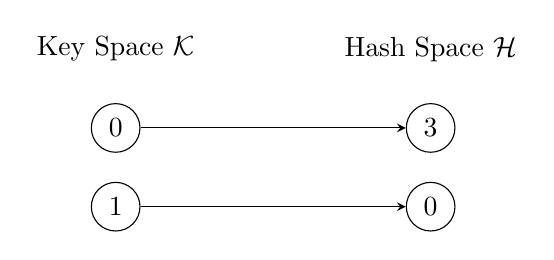
\begin{tikzpicture}[>=stealth]
            \node (A) at (0,2) {Key Space $\mathcal{K}$};
            \node (B) at (4,2) {Hash Space $\mathcal{H}$};
            \node[draw, circle] (k0) at (0,1) {$0$};
            \node[draw, circle] (h3) at (4,1) {$3$};
            \node[draw, circle] (k1) at (0,0) {$1$};
            \node[draw, circle] (h0) at (4,0) {$0$};
            \draw[->] (k0) -- (h3);
            \draw[->] (k1) -- (h0);
        \end{tikzpicture}
        \end{center}
    \end{proof}

    % Solution 27
    \item \textbf{Solution:}
    \begin{proof}
        We are given $M \equiv C \pmod p$ and $M \equiv C \pmod q$. By definition, $p \mid (M - C)$ and $q \mid (M - C)$. Since $p$ and $q$ are distinct primes, their greatest common divisor is $\gcd(p, q) = 1$. By the property of divisibility (an extension of Euclid's Lemma), if two coprime integers divide a number, their product also divides the number. Therefore, $pq \mid (M - C)$, which means $M \equiv C \pmod{pq}$.
    \end{proof}

    % Solution 28
    \item \textbf{Solution:}
    \begin{proof}
        We proceed by mathematical induction. \\
        \textbf{Base Case ($n=1$):} $X_1 \equiv a^1 X_0 + c \sum_{i=0}^{0} a^i = aX_0 + c(1) = aX_0 + c \pmod m$. This matches the recurrence definition. \\
        \textbf{Inductive Step:} Assume the formula holds for some arbitrary integer $k \ge 1$:
        \[ X_k \equiv a^k X_0 + c \sum_{i=0}^{k-1} a^i \pmod m \]
        We must show it holds for $k+1$. By the recurrence relation:
        \[ X_{k+1} \equiv aX_k + c \pmod m \]
        Substitute the inductive hypothesis into the equation:
        \[ X_{k+1} \equiv a \left( a^k X_0 + c \sum_{i=0}^{k-1} a^i \right) + c \pmod m \]
        Distribute the multiplier $a$:
        \[ X_{k+1} \equiv a^{k+1} X_0 + c \sum_{i=1}^{k} a^i + c \pmod m \]
        Absorb the isolated $c$ (which is $c \cdot a^0$) into the summation:
        \[ X_{k+1} \equiv a^{k+1} X_0 + c \sum_{i=0}^{k} a^i \pmod m \]
        This matches the closed-form formula for $n = k+1$. By mathematical induction, the formula holds for all $n \ge 1$.
    \end{proof}

    % Solution 29
    \item \textbf{Solution:}
    \begin{proof}
        Since $c=0$, the LCG closed-form simplifies to $X_n \equiv a^n X_0 \pmod m$. Assume for the sake of contradiction that there exists some $n \ge 1$ such that $X_n \equiv 0 \pmod m$. This implies:
        \[ m \mid (a^n X_0) \]
        Since $m$ is a prime, by Euclid's Lemma, $m$ must divide $a^n$ or $m$ must divide $X_0$. We are given that $X_0 \not\equiv 0 \pmod m$, so $m \nmid X_0$. Thus, it must be that $m \mid a^n$. Applying Euclid's Lemma repeatedly to $a^n$ implies that $m \mid a$. However, we are given that $a \not\equiv 0 \pmod m$, so $m \nmid a$. This is a logical contradiction. Therefore, the assumption that $X_n \equiv 0 \pmod m$ is false. The generator will never hit the zero state.
    \end{proof}

    % Solution 30
    \item \textbf{Solution:}
    \begin{proof}
        We first derive the necessary conditions for $m=12$. The prime factorization of 12 is $2^2 \times 3$. The prime factors are 2 and 3.
        \begin{enumerate}
            \item $\gcd(c, 12) = 1$. This implies $c$ must be coprime to 12. The possible values are $c \in \{1, 5, 7, 11\}$.
            \item $a-1$ must be divisible by all prime factors of $m$. Thus, $2 \mid (a-1)$ and $3 \mid (a-1)$. Since $\gcd(2,3)=1$, this implies $6 \mid (a-1)$.
            \item Since $m=12$ is divisible by 4, $a-1$ must be divisible by 4. Thus, $4 \mid (a-1)$.
        \end{enumerate}
        Combining conditions 2 and 3, $a-1$ must be a multiple of both 6 and 4. The least common multiple is $\text{lcm}(6, 4) = 12$. Therefore, $12 \mid (a-1)$, which means $a \equiv 1 \pmod{12}$.
        
        Now we evaluate the configuration $a=7, c=5$:
        \begin{itemize}
            \item $\gcd(5, 12) = 1$. (Condition 1 is met).
            \item $a-1 = 7-1 = 6$. The number 6 is divisible by 2 and 3. (Condition 2 is met).
            \item However, $4 \nmid 6$. (Condition 3 fails).
        \end{itemize}
        Because $a-1$ is not divisible by 4, the Hull-Dobell Theorem dictates that the generator will NOT have a full period. Therefore, $a=7, c=5$ is an invalid configuration for a full-period LCG modulo 12.
    \end{proof}

\end{enumerate}

\newpage

\section*{Concept Checklist \& Question Mapping (Repeated)}
\addcontentsline{toc}{section}{Concept Checklist \& Question Mapping (Repeated)}
For ease of reference, the concept mapping is repeated below:

\begin{itemize}
    \item \textbf{C1: Direct Algebraic Manipulation} (Definition of Congruence, Substitution, Repackaging) $\implies$ \textit{Tested in Problems 1, 2, 3, 4, 5}
    \item \textbf{C2: Exhaustive Residue Checking / Proof by Cases} (Division Algorithm, Small Moduli Heuristic) $\implies$ \textit{Tested in Problems 6, 7, 8, 9, 10}
    \item \textbf{C3: Biconditional Parity and Modulus Reduction} (Contrapositive for ``OR'', Parity Constraints) $\implies$ \textit{Tested in Problems 11, 12, 13, 18, 19}
    \item \textbf{C4: Difference of Squares \& Algebraic Expansion} (Polynomial factoring) $\implies$ \textit{Tested in Problems 2, 12, 13, 16}
    \item \textbf{C5: Adding Zero / Telescoping} (Bridging variables) $\implies$ \textit{Tested in Problems 3, 28}
    \item \textbf{C6: Modulus Factoring \& Divisibility Properties} (If $kn \mid km$, then $n \mid m$) $\implies$ \textit{Tested in Problems 4, 14, 17}
    \item \textbf{C7: Cancellation Law \& Coprime Conditions} (Euclid's Lemma) $\implies$ \textit{Tested in Problems 15, 26, 27, 29}
    \item \textbf{C8: Equivalence Relation Properties} (Reflexive, Symmetric, Transitive) $\implies$ \textit{Tested in Problem 3}
    \item \textbf{C9: Polynomial Congruence Properties} $\implies$ \textit{Tested in Problem 20}
    \item \textbf{C10: Abstract Real-World Modeling} (Linear Congruential Generators, Hash Tables, RSA Cryptography) $\implies$ \textit{Tested in Problems 26, 27, 28, 29, 30}
    \item \textbf{C11: Identifying Logical Flaws} (Division Fallacy, Exponent Fallacy, Square Root Fallacy) $\implies$ \textit{Tested in Problems 21, 22, 23, 24, 25}
\end{itemize}

\end{document}